\documentclass[a4paper, 12pt]{article}

% Pacotes essenciais
\usepackage{subcaption}
\usepackage[utf8]{inputenc}    % Suporte a caracteres UTF-8
\usepackage[brazil]{babel}     % Idioma em português brasileiro
\usepackage{amsmath, amssymb}  % Pacotes matemáticos
\usepackage{graphicx}          % Inclusão de imagens
\usepackage{geometry}          % Ajuste de margens
\usepackage[utf8]{inputenc}
\usepackage{amsmath, amssymb, amsfonts}
\usepackage{graphicx}
\usepackage{float}
\usepackage{hyperref}
\usepackage{geometry}
\geometry{top=2.5cm, bottom=2.5cm, left=2.5cm, right=2.5cm}

% Personalização de cabeçalho e rodapé
\usepackage{fancyhdr}
\pagestyle{fancy}
\fancyhf{}
\fancyhead[L]{Tópicos de Física Teórica I}
\fancyhead[R]{\thepage}
\fancyfoot[C]{\small Universidade Federal de Fortaleza - Departamento de Física}

% Título e autorssaes
\title{\textbf{1° Lista}}
\author{
    Carlos Miguel Moreira Gonçalves \\
    Igor Pereira Cavalcante \\
    Robert Bertoldo Tavares \\
}
\date{\today}

\begin{document}

\maketitle
\thispagestyle{fancy}

\section*{Problema 1}
Considerando a distribuição de Boltzmann para o problema do oscilador harmônico \textbf{clássico}, temos:

\begin{equation}
P(x) \propto e^{-\beta E(x)}, \quad \text{com } E(x) = \frac{1}{2} k x^2,
\end{equation}

onde \(\beta = \frac{1}{k_B T}\). Para gerar valores aleatórios de \(x\) que sigam essa distribuição, utilizamos o método de rejeição. Nesse método, valores de \(x\) são inicialmente sorteados a partir de uma distribuição uniforme e aceitos com probabilidade proporcional a \(P(x)\). Essa abordagem funciona porque a probabilidade de aceitação é ajustada para refletir a forma de \(P(x)\), garantindo que valores associados a maior probabilidade (maior \(P(x)\)) têm maior chance de serem aceitos, enquanto valores menos prováveis são rejeitados. Assim, a amostra gerada reflete fielmente a distribuição de Boltzmann.

\subsection*{a), b), c) e f)}

Sorteamos valores aleatórios de \(x\), como descrito anteriormente, e em seguida criamos um histograma dos valores sorteados e o normalizamos.

\begin{figure}[H]
    \centering
    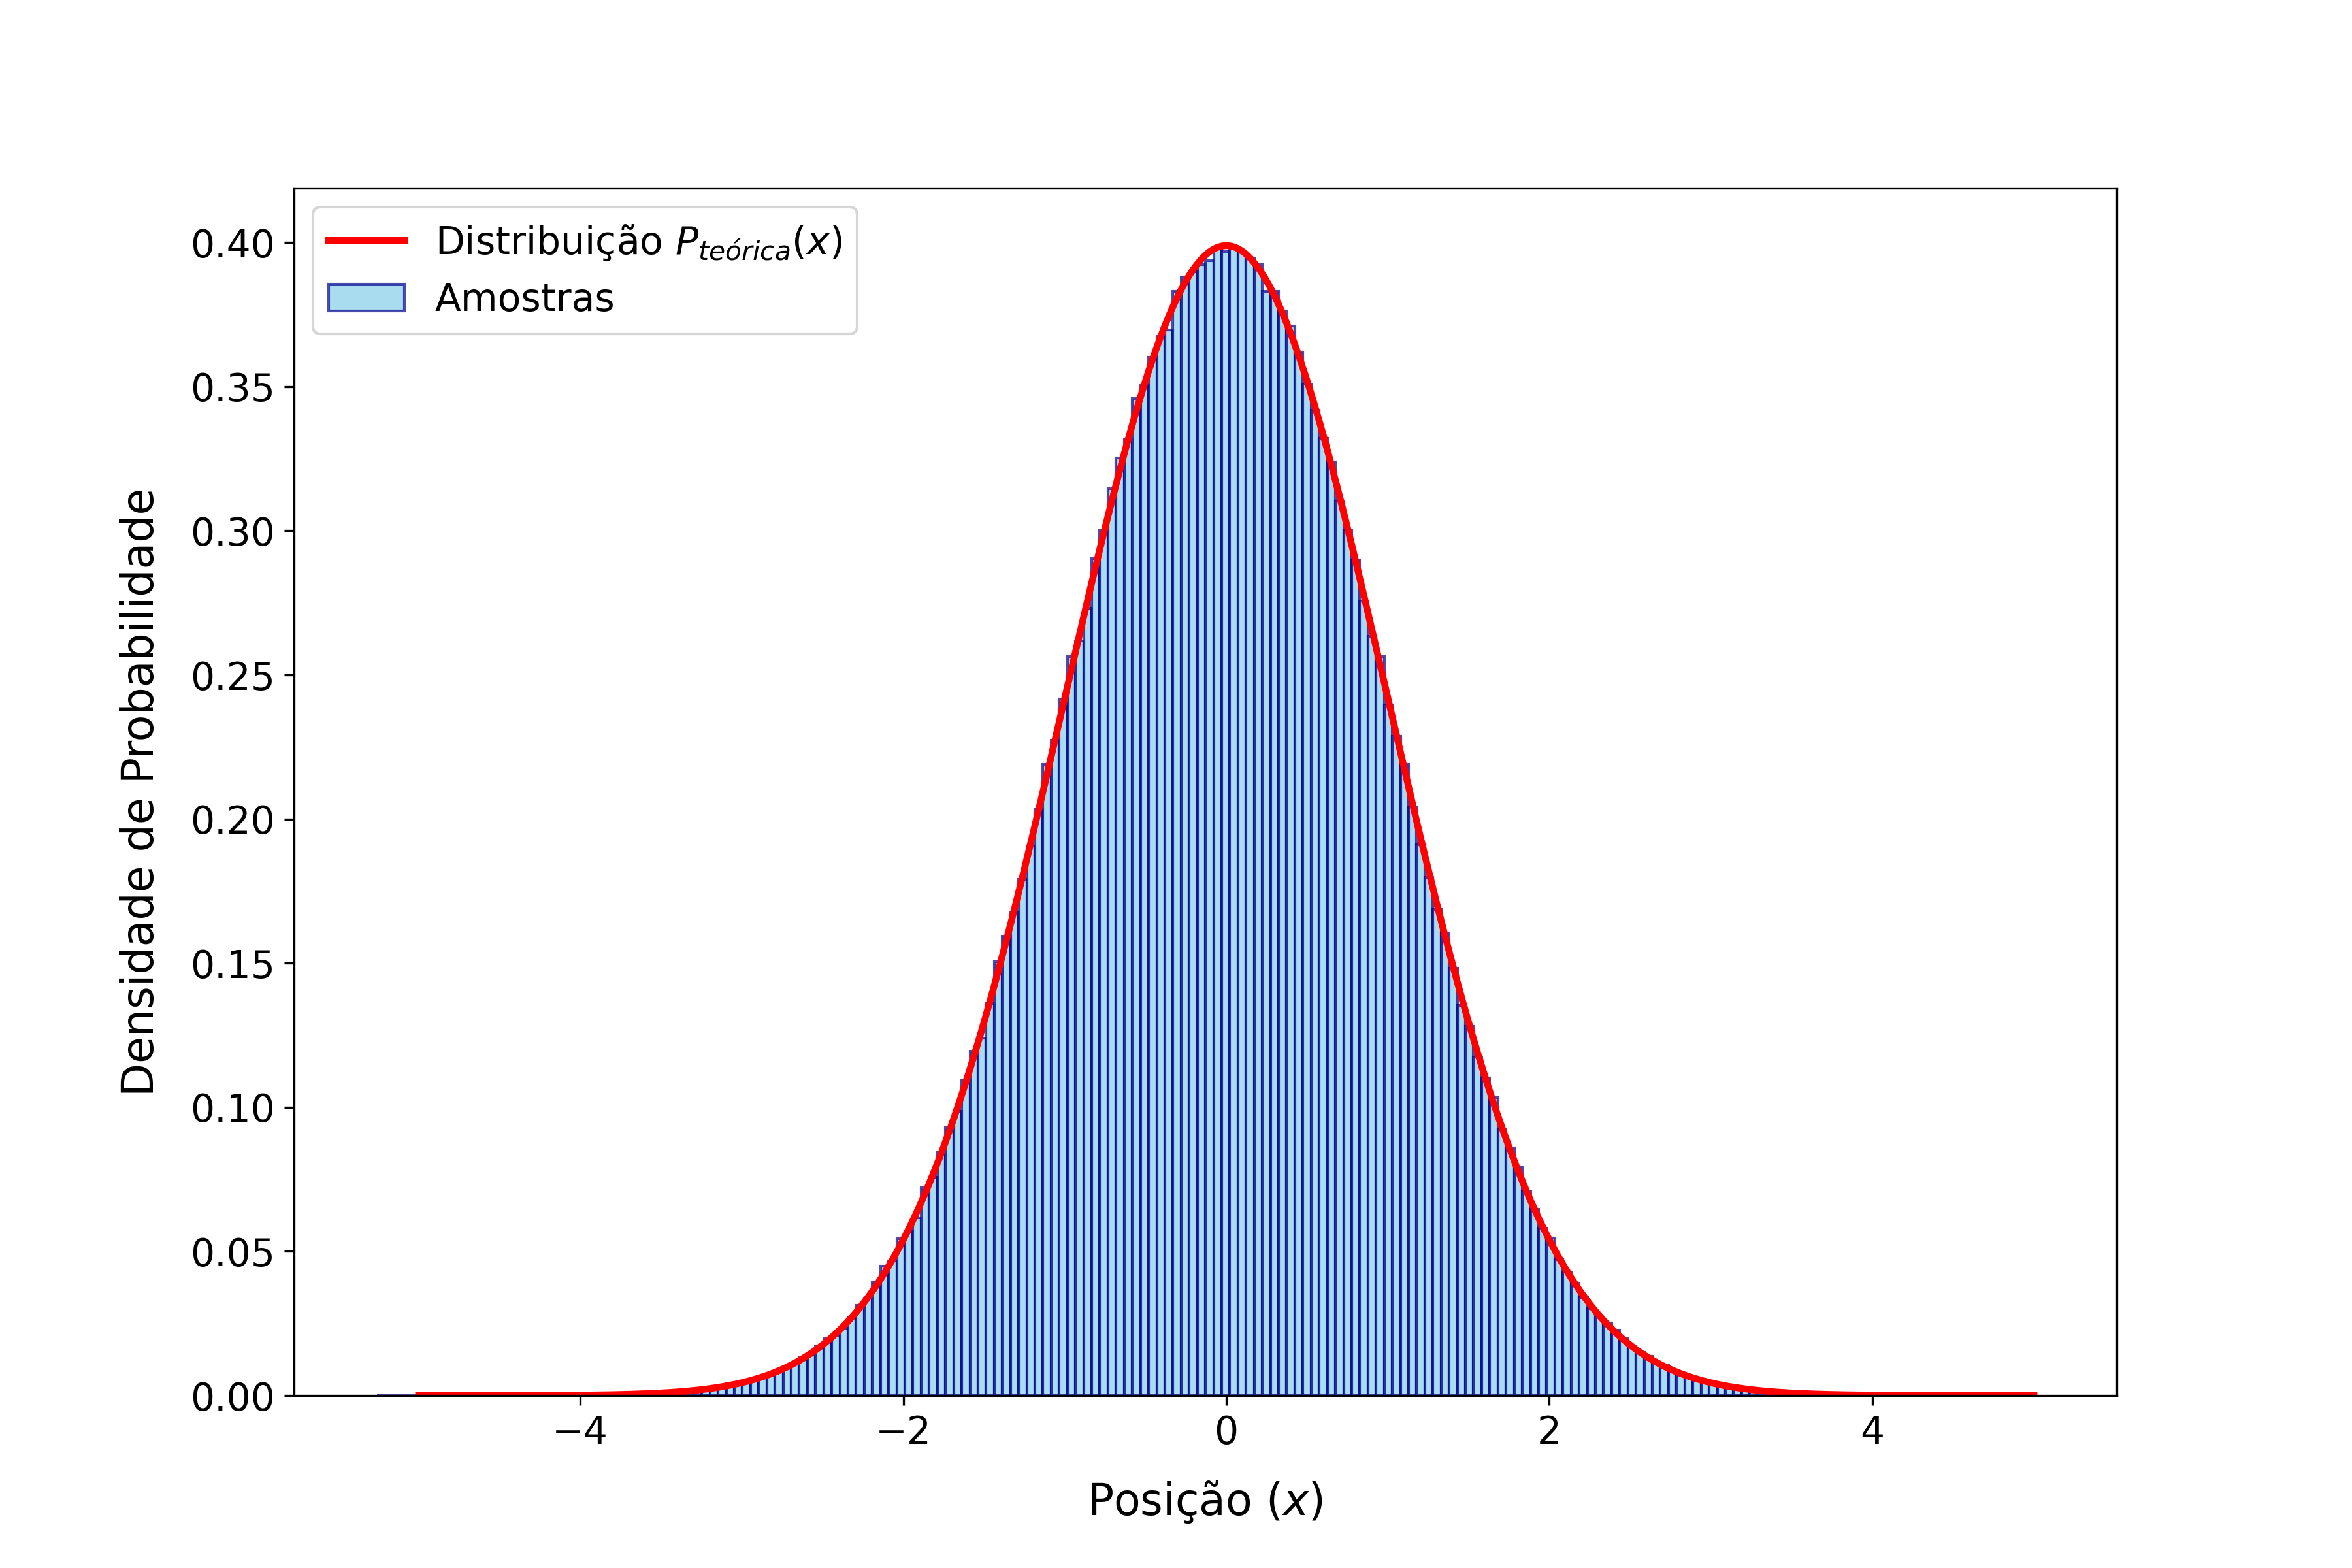
\includegraphics[scale=0.39]{Q1_a.png}
    \caption{Gráfico da distribuição de Boltzmann (linha contínua vermelha), comparando com a distribuição gerada a partir do método de rejeição (barras azuis).}
    \label{fig:Q1_a}
\end{figure}

Na Fig. \ref{fig:Q1_a}, sobrepomos a curva empírica com a curva teórica da distribuição de Boltzmann, dada por:
\begin{equation}
P_{\text{teórica}}(x) = \sqrt{\frac{\beta k}{2 \pi}} \exp \left( -\frac{\beta k x^2}{2} \right).
\end{equation}

\subsection*{d) e e)}

Para avaliar quantitativamente se as amostras que obtivemos com o sorteio pelo método da rejeição são consistentes com a distribuição teórica, calculamos a média e a variância, dadas por: 
\begin{equation}
\mathbb{E}[x] = 0, \quad \text{Var}(x) = \frac{1}{\beta k}.
\end{equation}

\begin{table}[H]
\centering
\begin{tabular}{|c|c|c|c|}
\hline
\textbf{Parâmetro} & \textbf{Valor Encontrado} & \textbf{Valor Teórico} & \textbf{Erro (\%)} \\ \hline
Média              & -0.00122                  & 0                      & 0.1224             \\ \hline
Variância          & 0.99988                   & 1.0                    & 0.0124             \\ \hline
\end{tabular}
\caption{Comparação entre valores encontrados nas simulações e os valores teóricos.}
\label{tab:media_variancia}
\end{table}

Realizamos ainda os testes estatísticos de Kolmogorov-Smirnov (K-S). Os resultados estão na Tabela \ref{tab:teste_ks}.

\begin{table}[H]
\centering
\begin{tabular}{|l|c|}
\hline
\textbf{Parâmetro} & \textbf{Valor} \\ \hline
$D$                & 0.00106        \\ \hline
$D_{critico}$      & 0.00135        \\ \hline
$p_{valor}$        & 0.20624        \\ \hline
\end{tabular}
\caption{Resultados do teste K-S.}
\label{tab:teste_ks}
\end{table}

O parâmetro \(D\) é pequeno, indicando que a diferença absoluta entre a função de distribuição empírica da amostra (EDF) e a função de distribuição acumulada teórica (CDF) é muito baixa. Isso demonstra uma forte concordância entre a amostra sorteada e a distribuição teórica. Como \(D \leq D_{critico}\), não podemos rejeitar a hipótese nula (\(H_0\)), indicando que não há evidências estatísticas para rejeitar que os dados sigam a distribuição teórica.

\section*{Questão 2}

Dado um sistema biestável, com um potencial dado por:
\begin{equation}
V(x) = x^4 - 4x^2,
\end{equation}
que possui dois mínimos estáveis e uma barreira entre eles. A dinâmica de uma partícula sujeita a esse potencial, na presença de ruído térmico, é governada pela equação de Langevin:

\begin{equation}
\frac{dx}{dt} = -\frac{1}{\gamma} \frac{dV}{dx} + \eta(t),
\end{equation}
onde \(\gamma\) é o coeficiente de amortecimento e \(\eta(t)\) é um ruído Gaussiano com média zero e correlação \(\langle \eta(t) \eta(t') \rangle = 2D \delta(t - t')\). Essa equação pode ser resolvida numericamente para simular a dinâmica da partícula.

\subsection*{a)}

Simulamos a dinâmica resolvendo numericamente a equação. Consideramos que o sistema atinge equilíbrio quando a diferença entre os passos é consistentemente muito pequena (tolerância de \(10^{-8}\)). Para evitar tempos de simulação muito longos, fixamos uma temperatura muito baixa (\(\beta = 10\), equivalente a \(D = 10^{-7}\)). Nesse regime, a partícula fica confinada em um dos mínimos. Realizamos 100 simulações e plotamos a distribuição de posições, comparando com a distribuição de Boltzmann:

\begin{figure}[H]
    \centering
    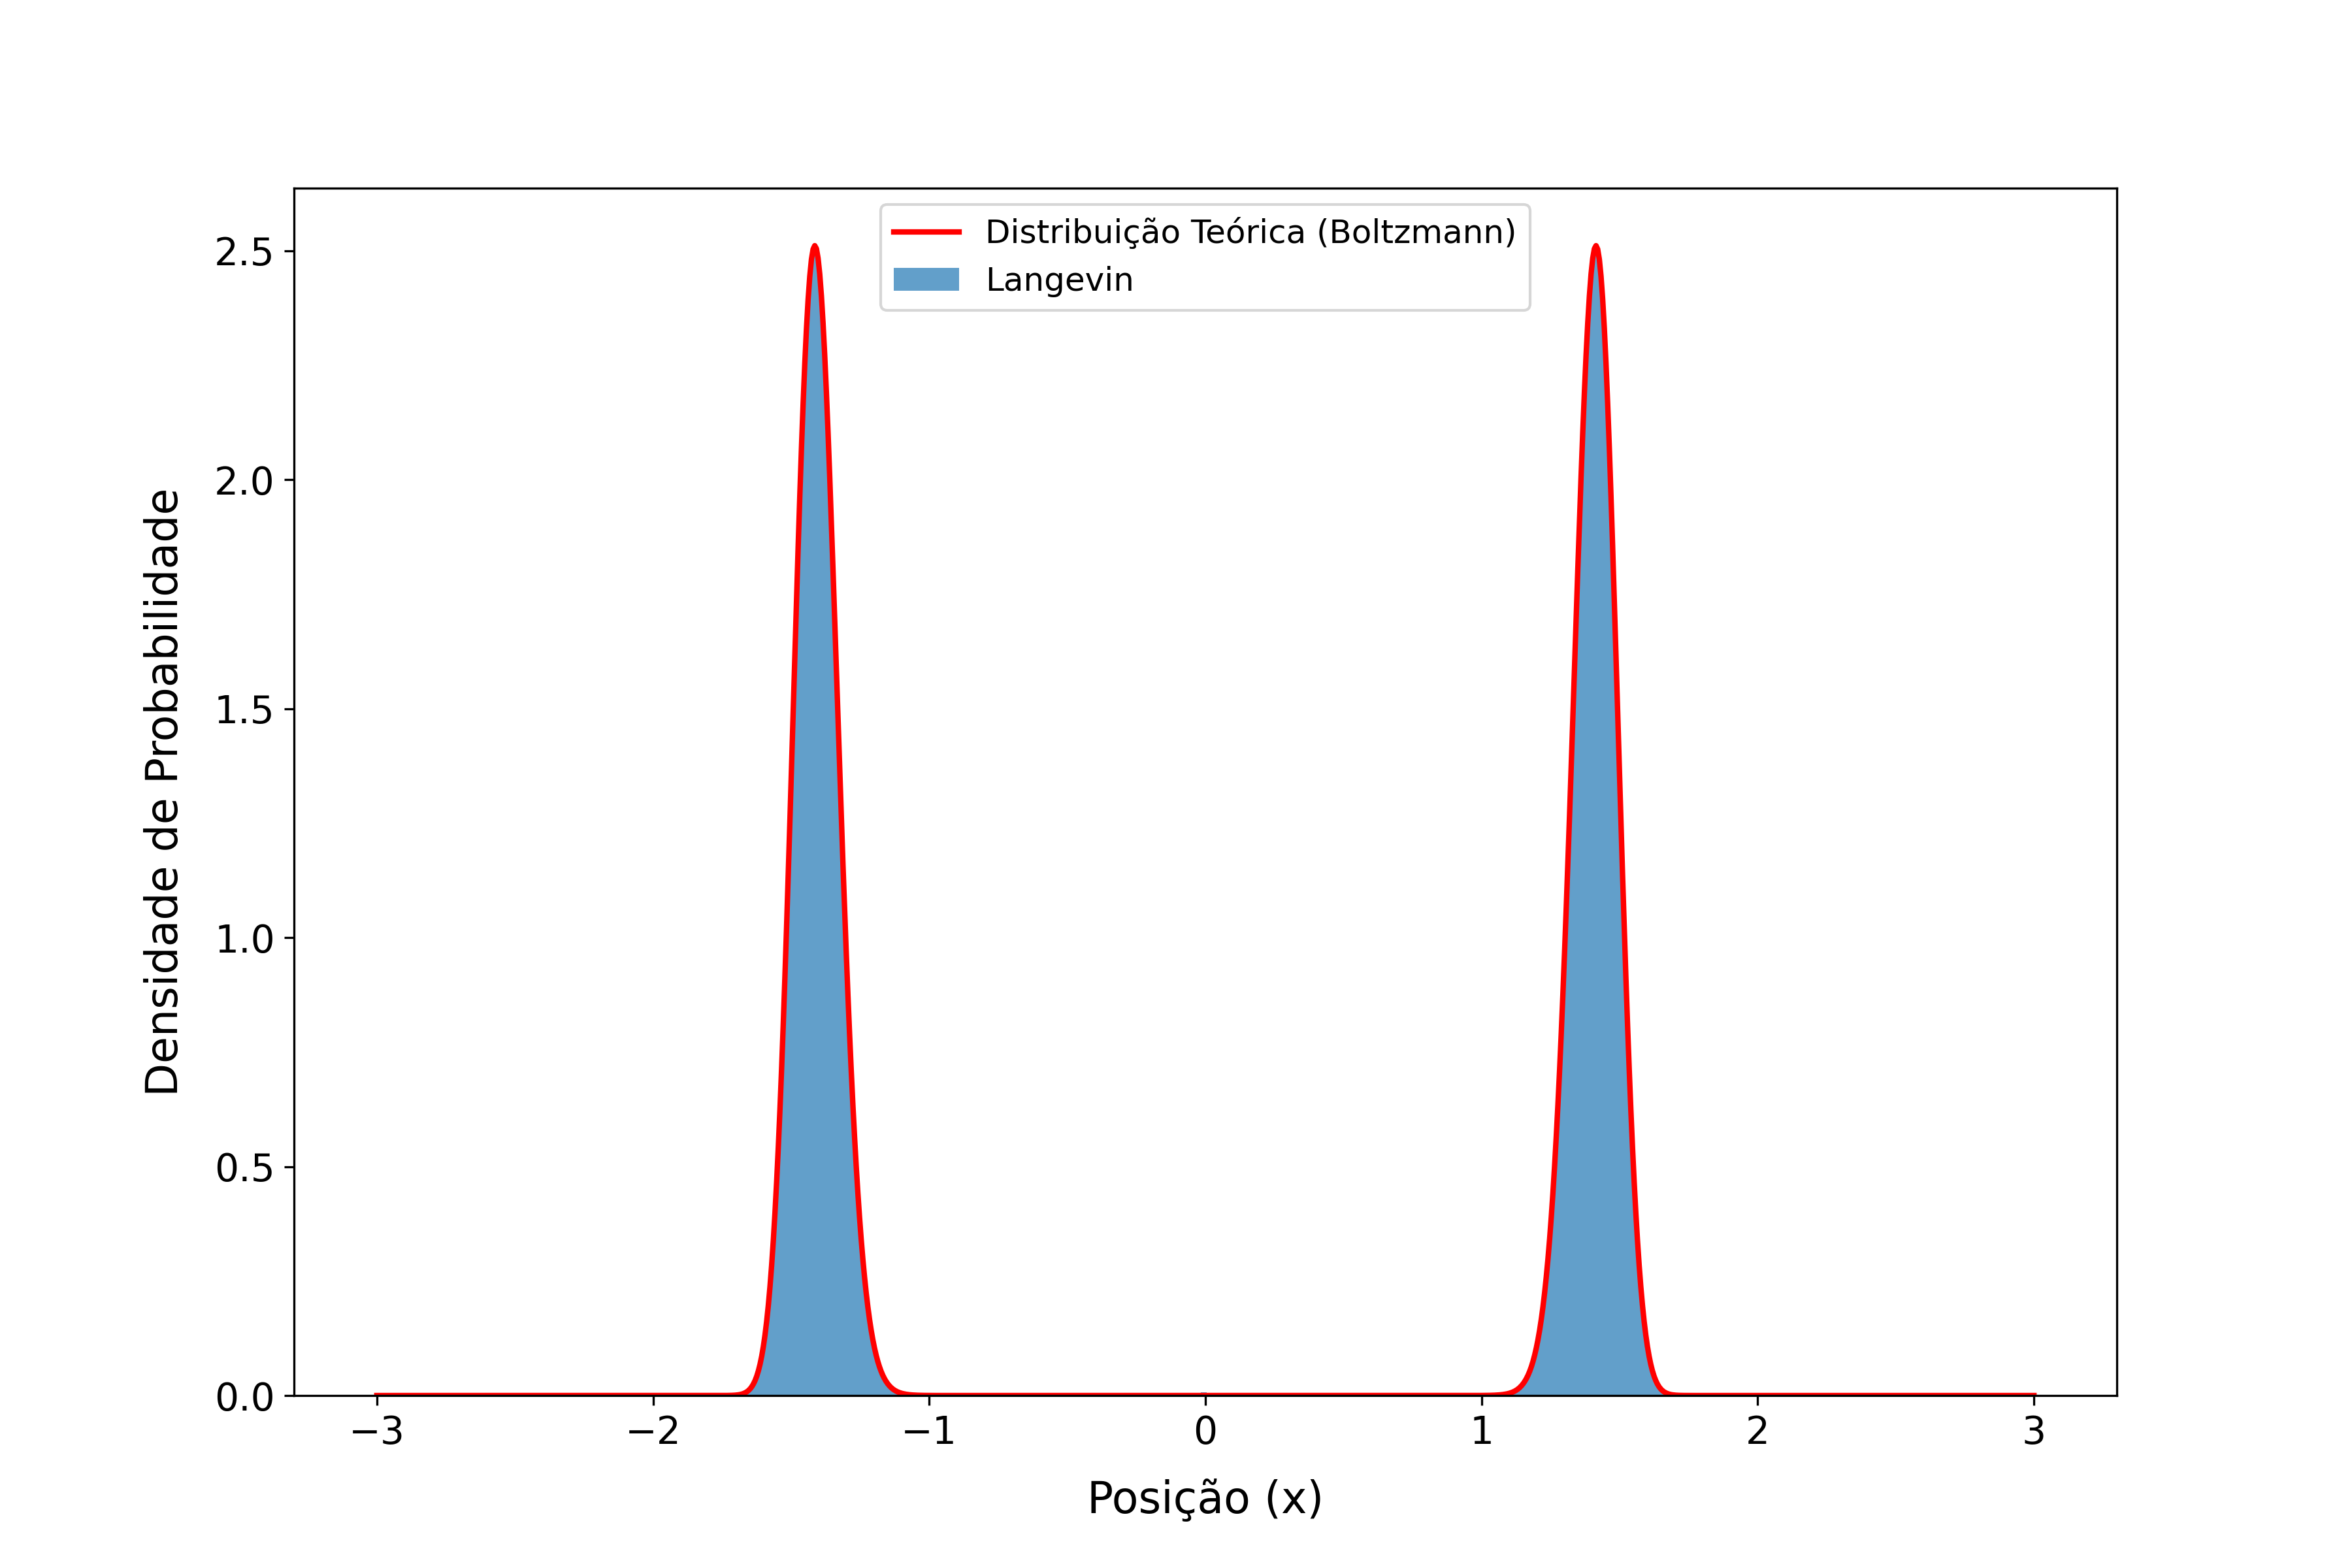
\includegraphics[scale=0.39]{Q2_a.png}
    \caption{Gráfico da distribuição de Boltzmann (linha contínua vermelha) comparada à distribuição gerada pela dinâmica da equação de Langevin (barras azuis).}
    \label{fig:Q2_a}
\end{figure}

\subsection*{b)}

Utilizamos o algoritmo de Metropolis para simular o comportamento estatístico da partícula no potencial. Inicialmente, sorteamos uma posição inicial \(x_0\). Em cada passo, propomos uma nova posição \(x_{\text{nova}} = x + \Delta x\), com \(\Delta x\) gerado de uma distribuição uniforme. A nova posição é aceita com probabilidade:
\begin{equation}
P = \min(1, e^{-\beta \Delta V}),
\end{equation}
onde \(\Delta V = V(x_{\text{nova}}) - V(x)\). Caso não seja aceita, a posição permanece em \(x\).

\begin{figure}[H]
    \centering
    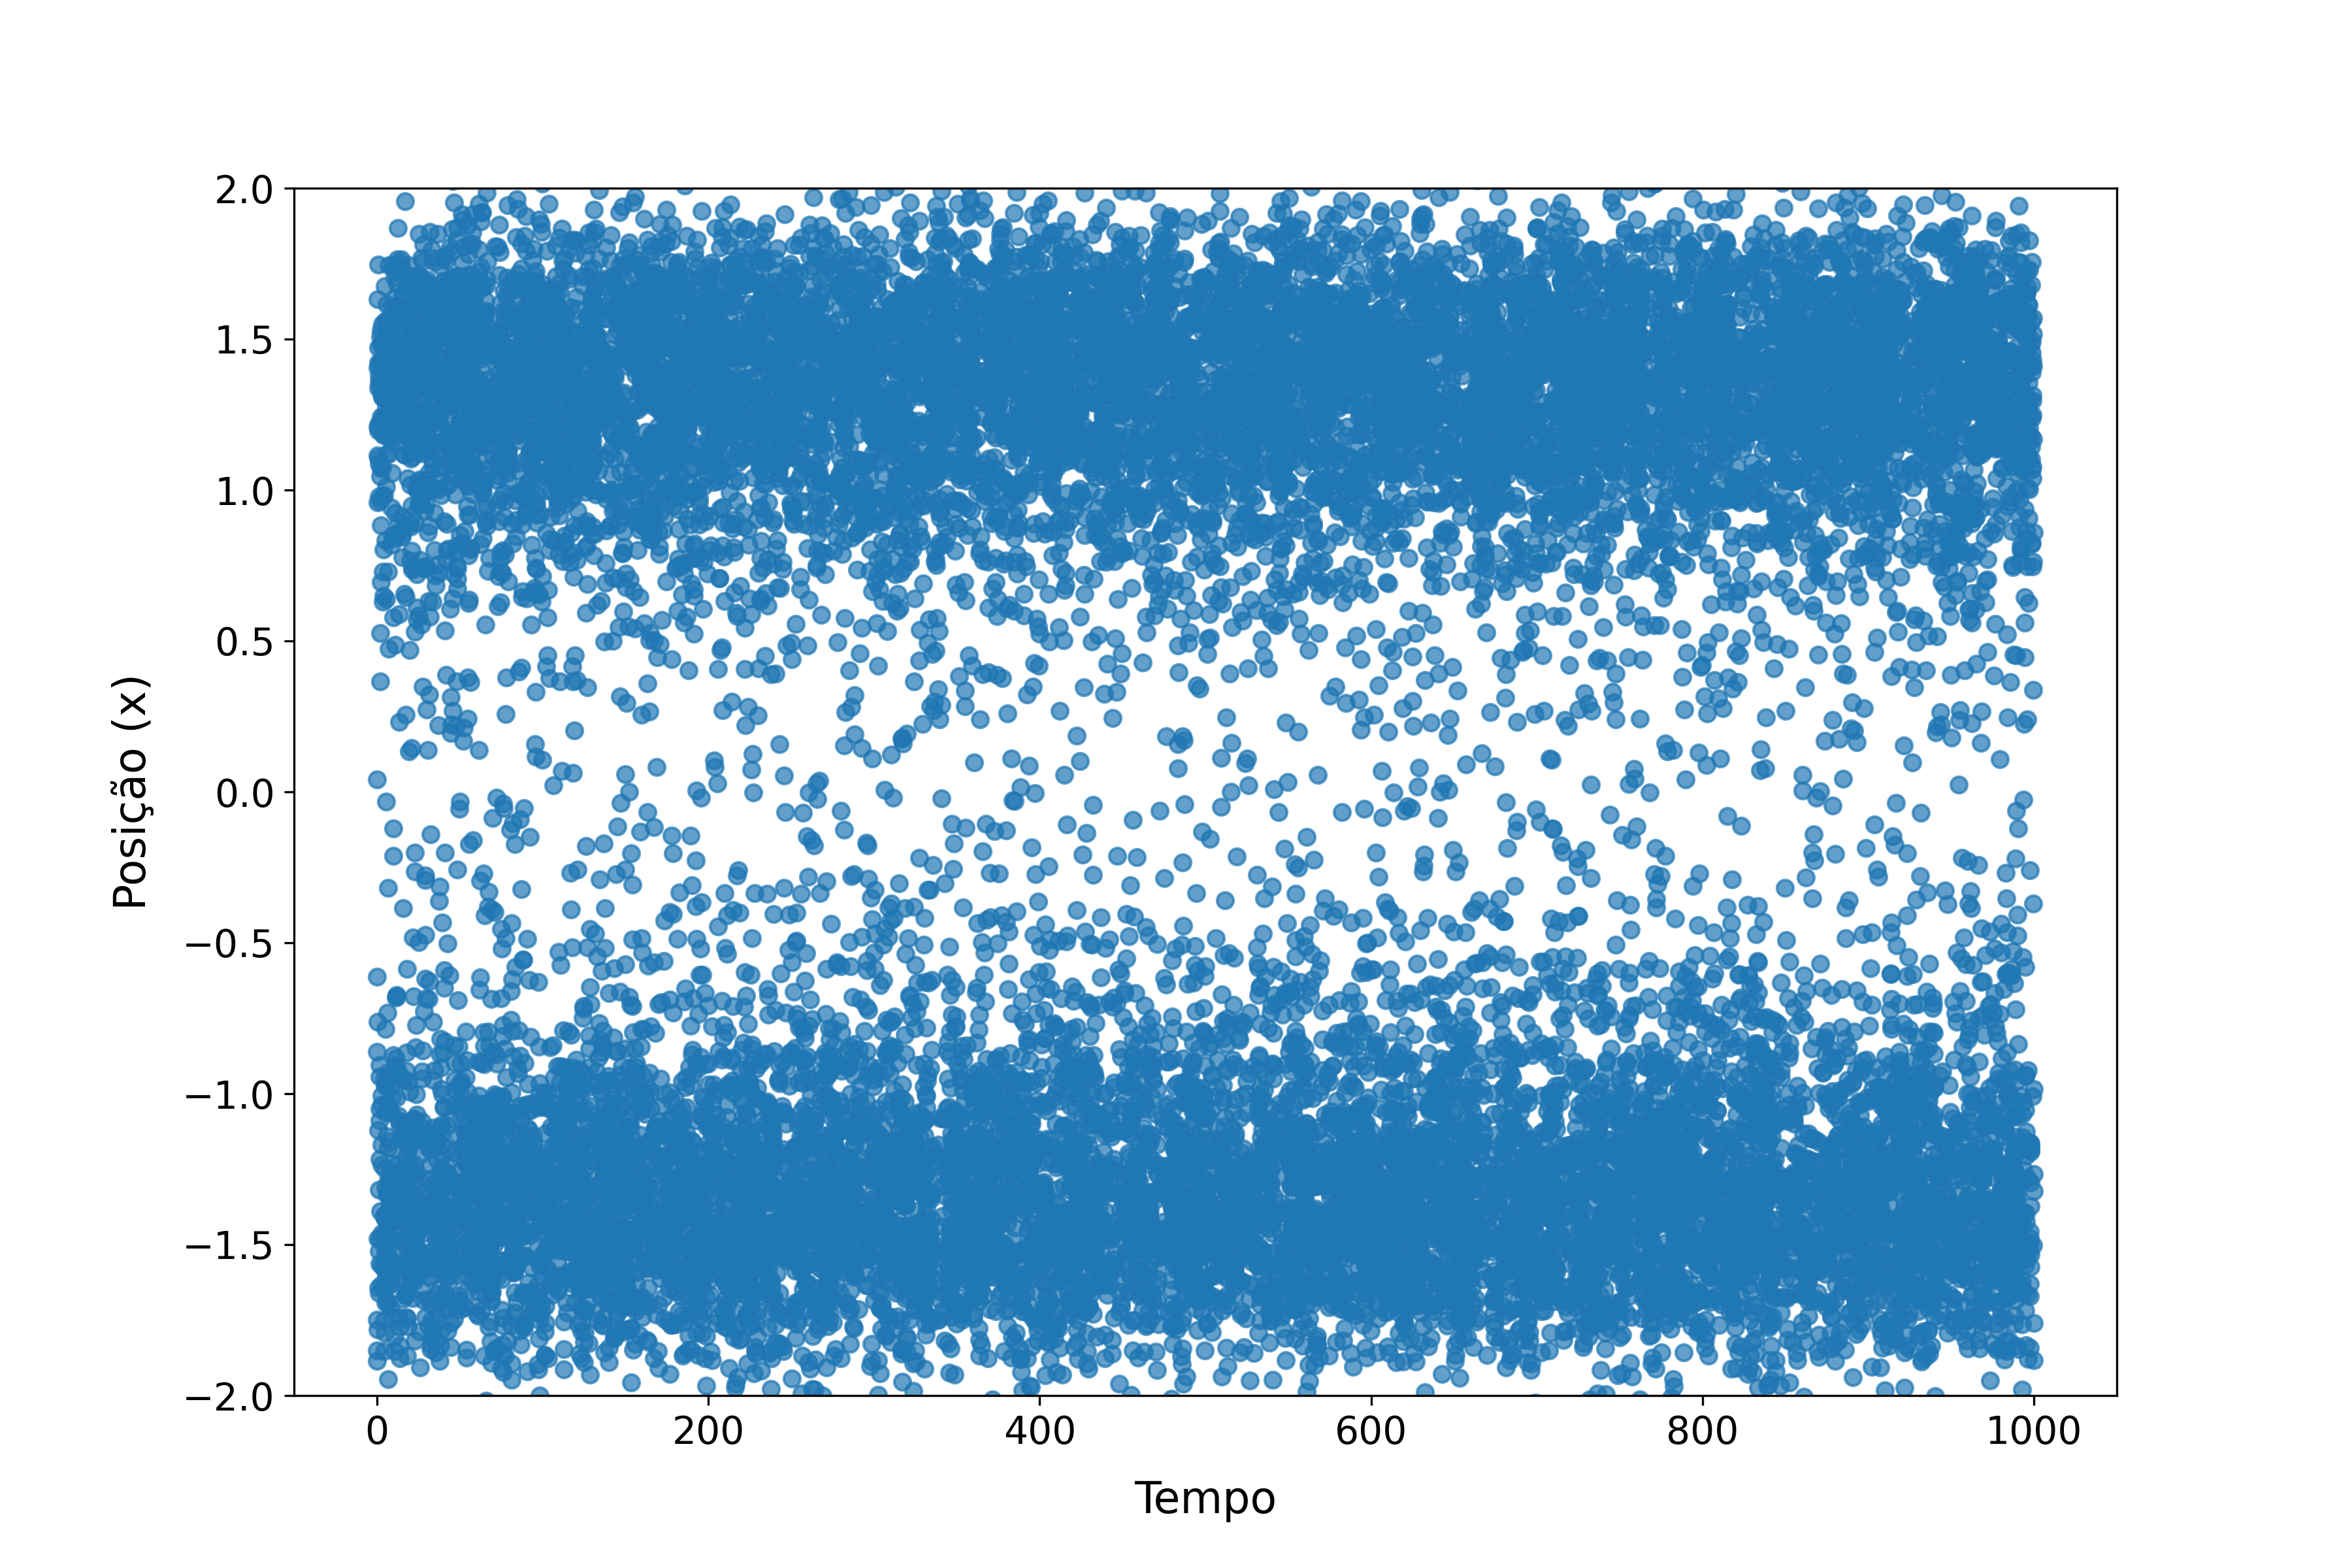
\includegraphics[scale=0.39]{Q2_b.png}
    \caption{Gráfico da posição em função do tempo para uma simulação de Metropolis. \(\beta = 0.8\), \(dx = 0.7\).}
    \label{fig:Q2_b}
\end{figure}

Abaixo, apresentamos o histograma da distribuição de posições:
\begin{figure}[H]
    \centering
    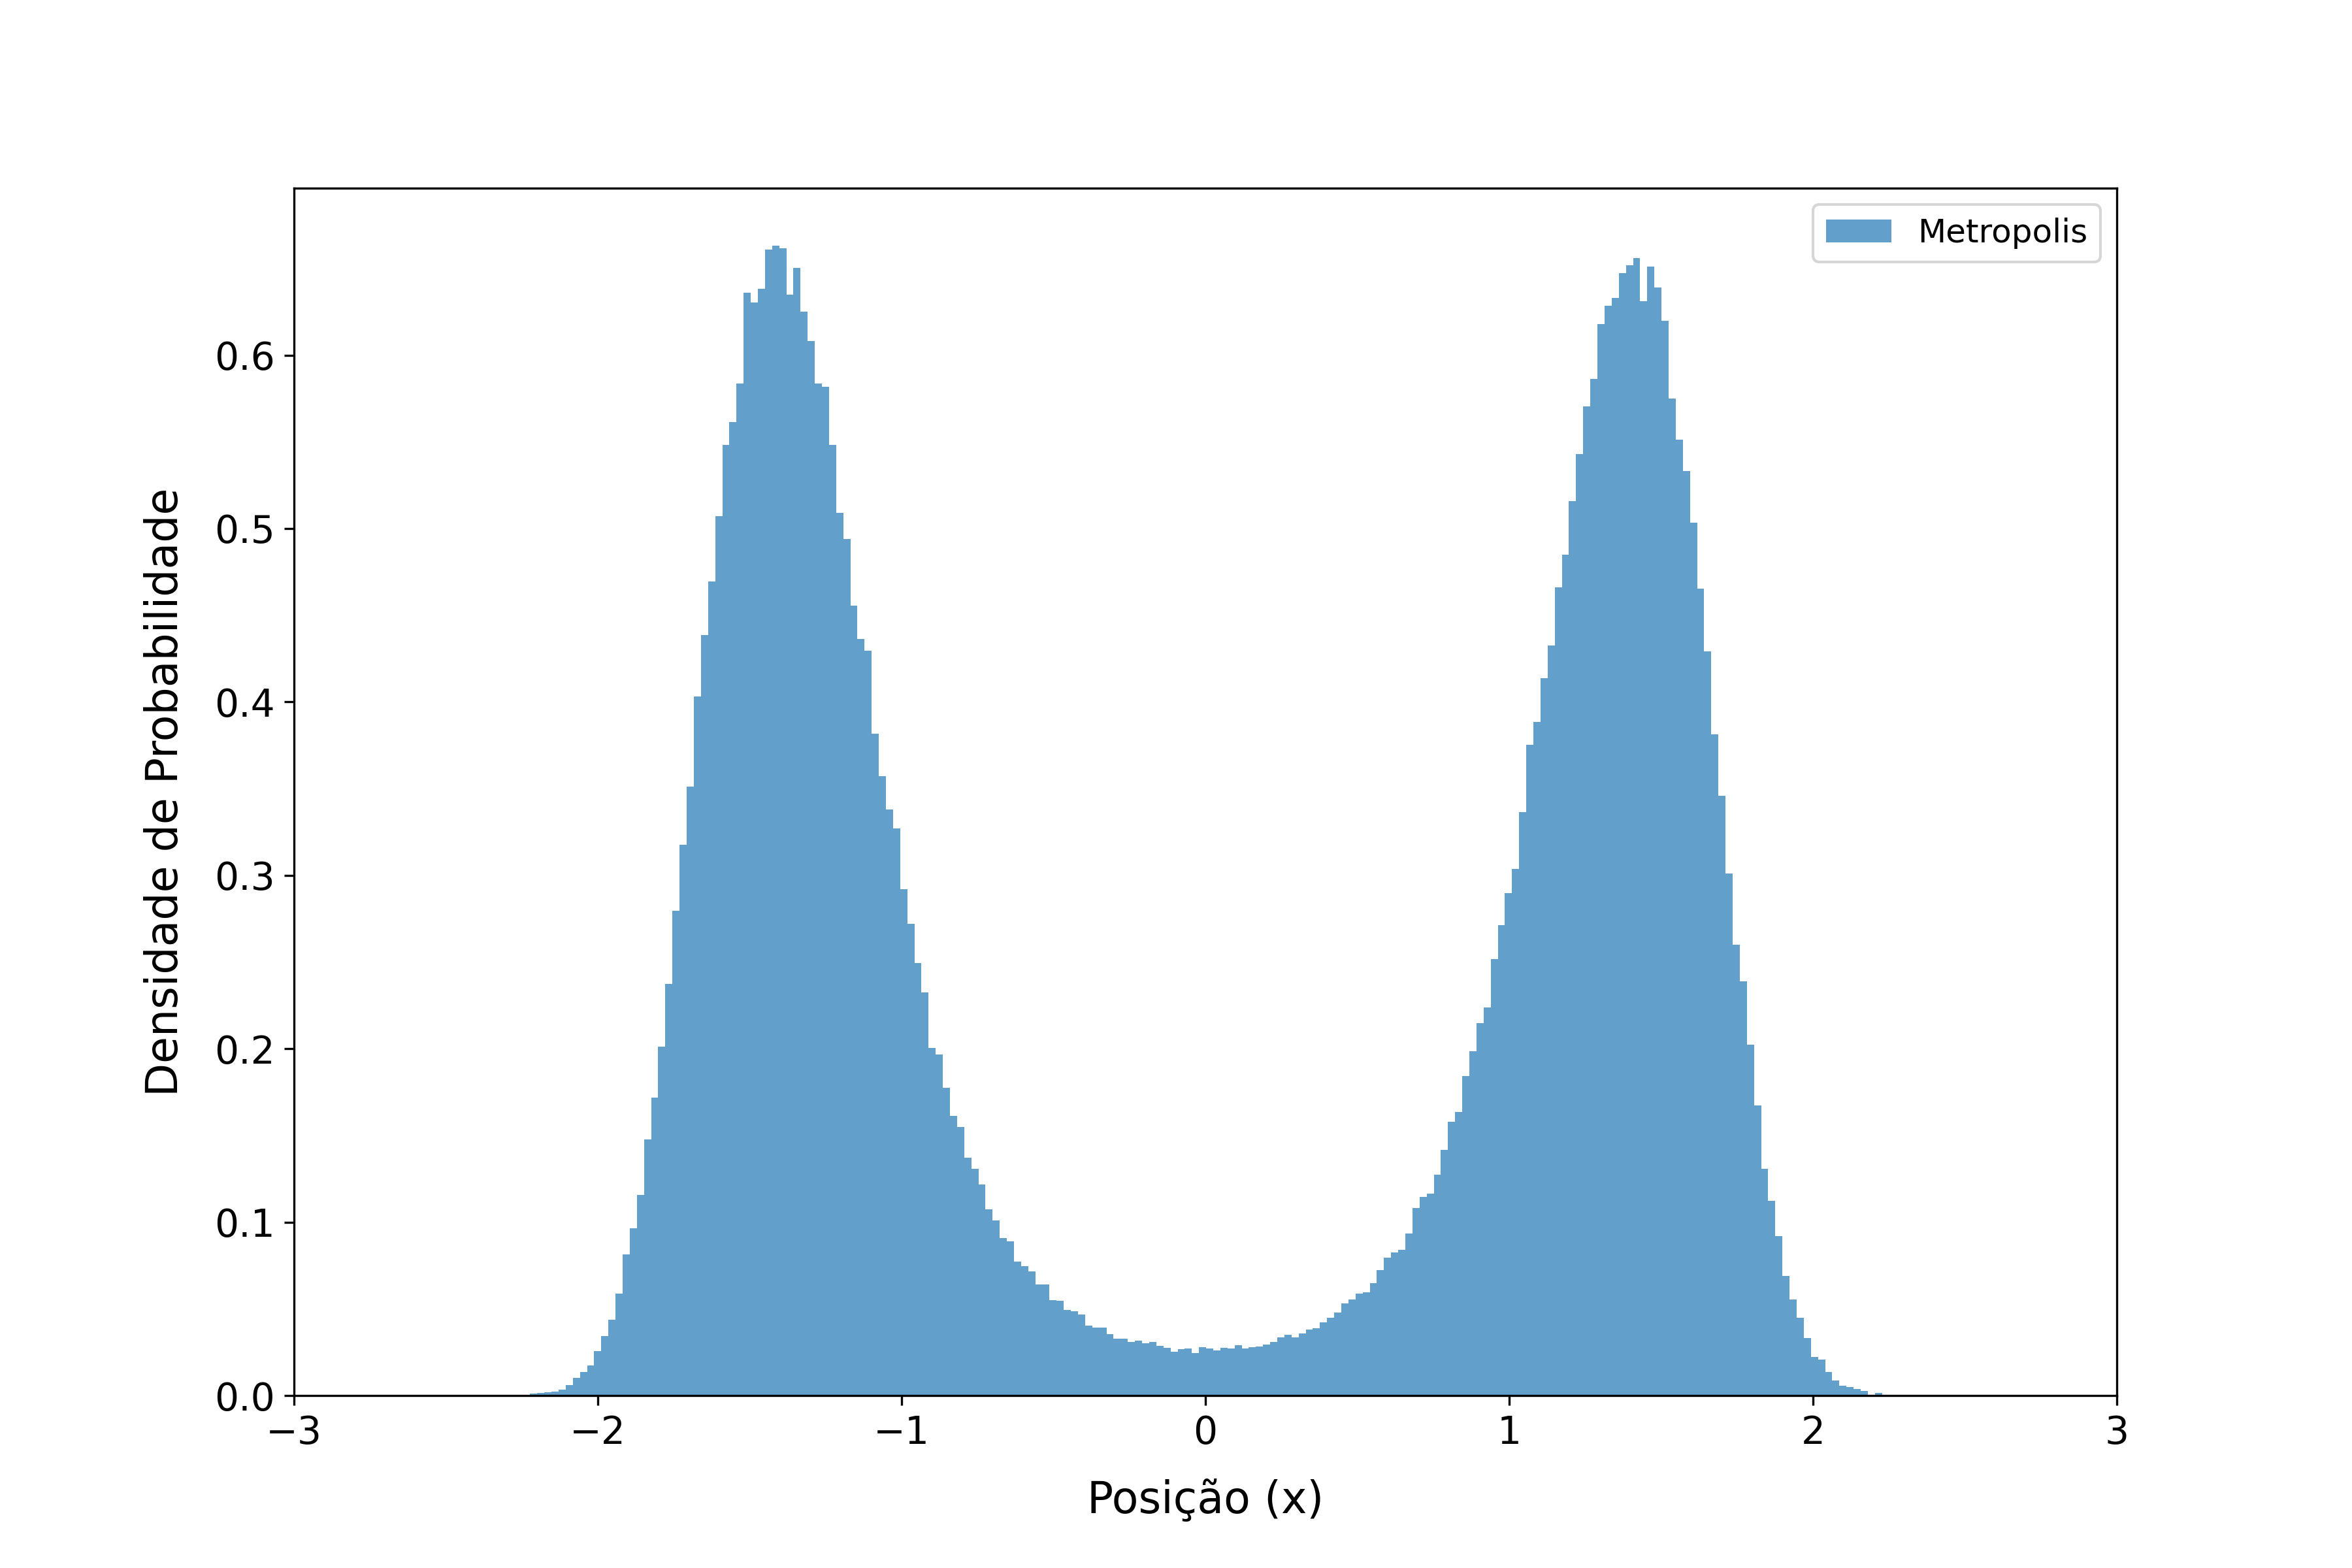
\includegraphics[scale=0.39]{Q2_b2.png}
    \caption{Histograma da distribuição de posições na simulação de Metropolis. \(\beta = 0.8\), \(dx = 0.7\).}
    \label{fig:Q2_b2}
\end{figure}

\subsection*{c)}

Ao comparar as simulações de Metropolis com a dinâmica de Langevin, as distribuições são muito semelhantes, conforme mostrado na Fig. \ref{fig:Q2_c}.

\begin{figure}[H]
    \centering
    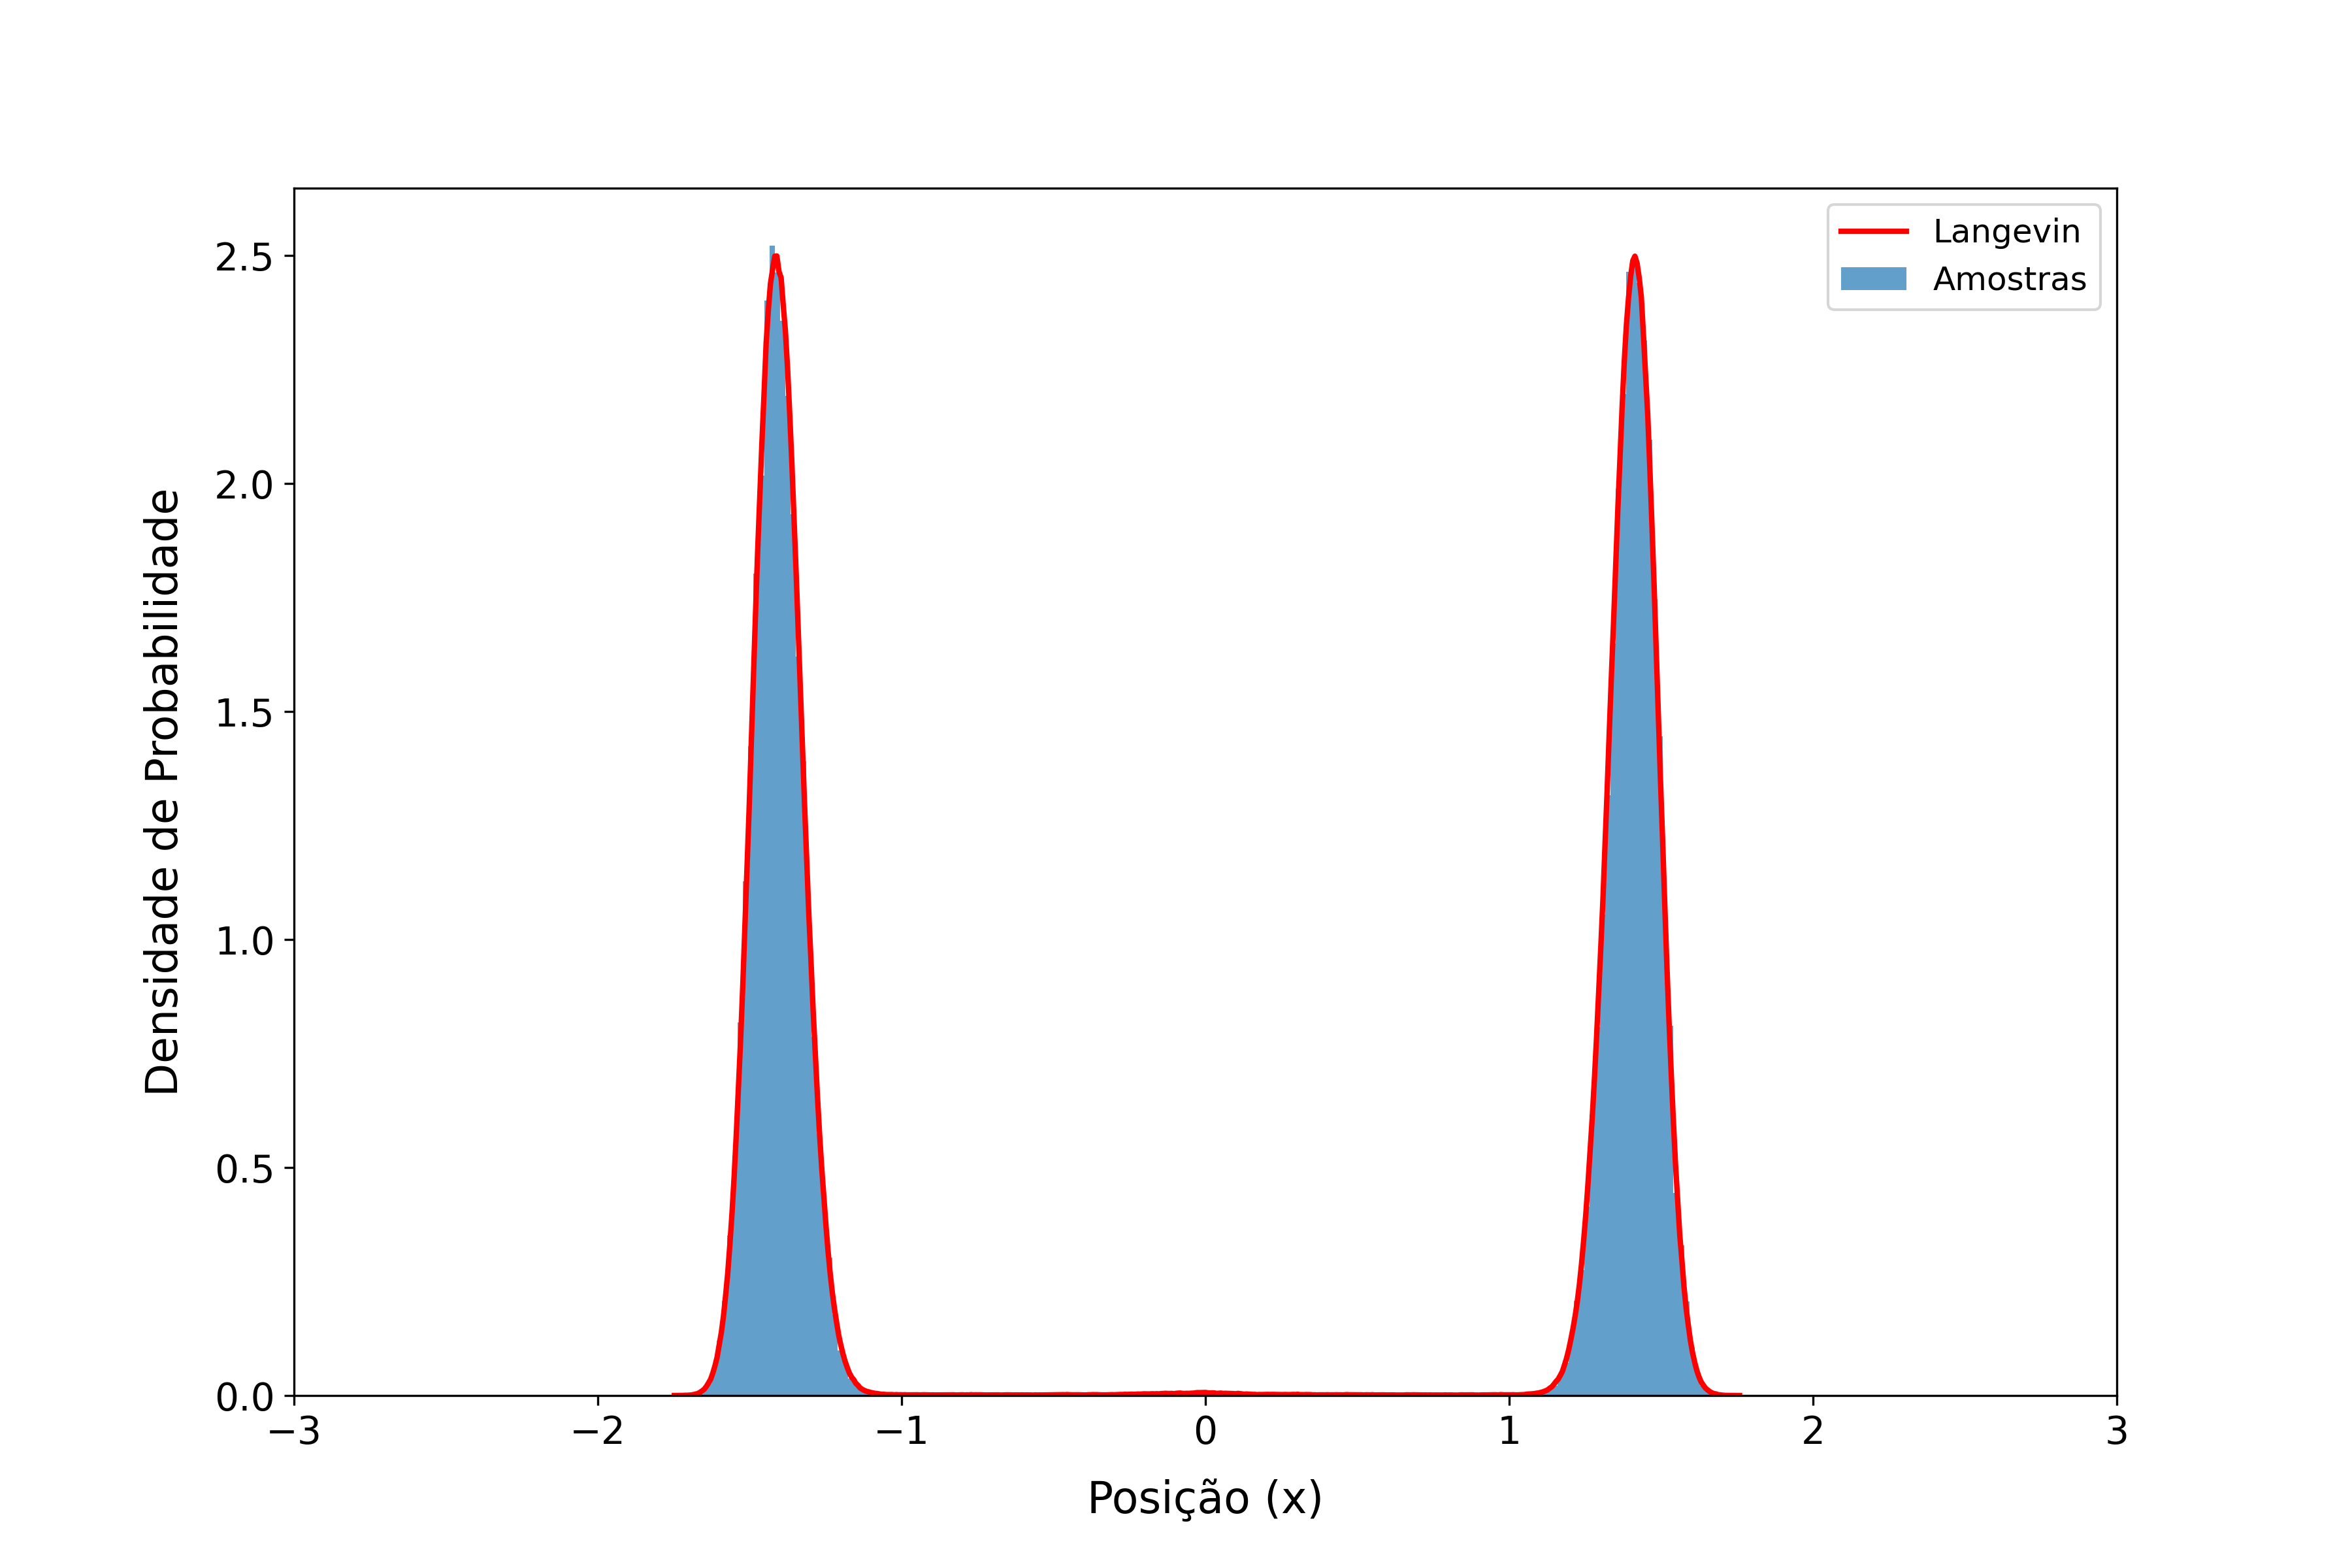
\includegraphics[scale=0.39]{Q2_c.png}
    \caption{Distribuição da dinâmica de Langevin (linha contínua vermelha) comparada com a distribuição gerada por Metropolis (barras azuis).}
    \label{fig:Q2_c}
\end{figure}

Por fim, ao variar \(\beta\), podemos analisar a probabilidade de encontrar a partícula próxima aos mínimos. Esse comportamento está apresentado na Fig. \ref{fig:Q2_d}.

\begin{figure}[H]
    \centering
    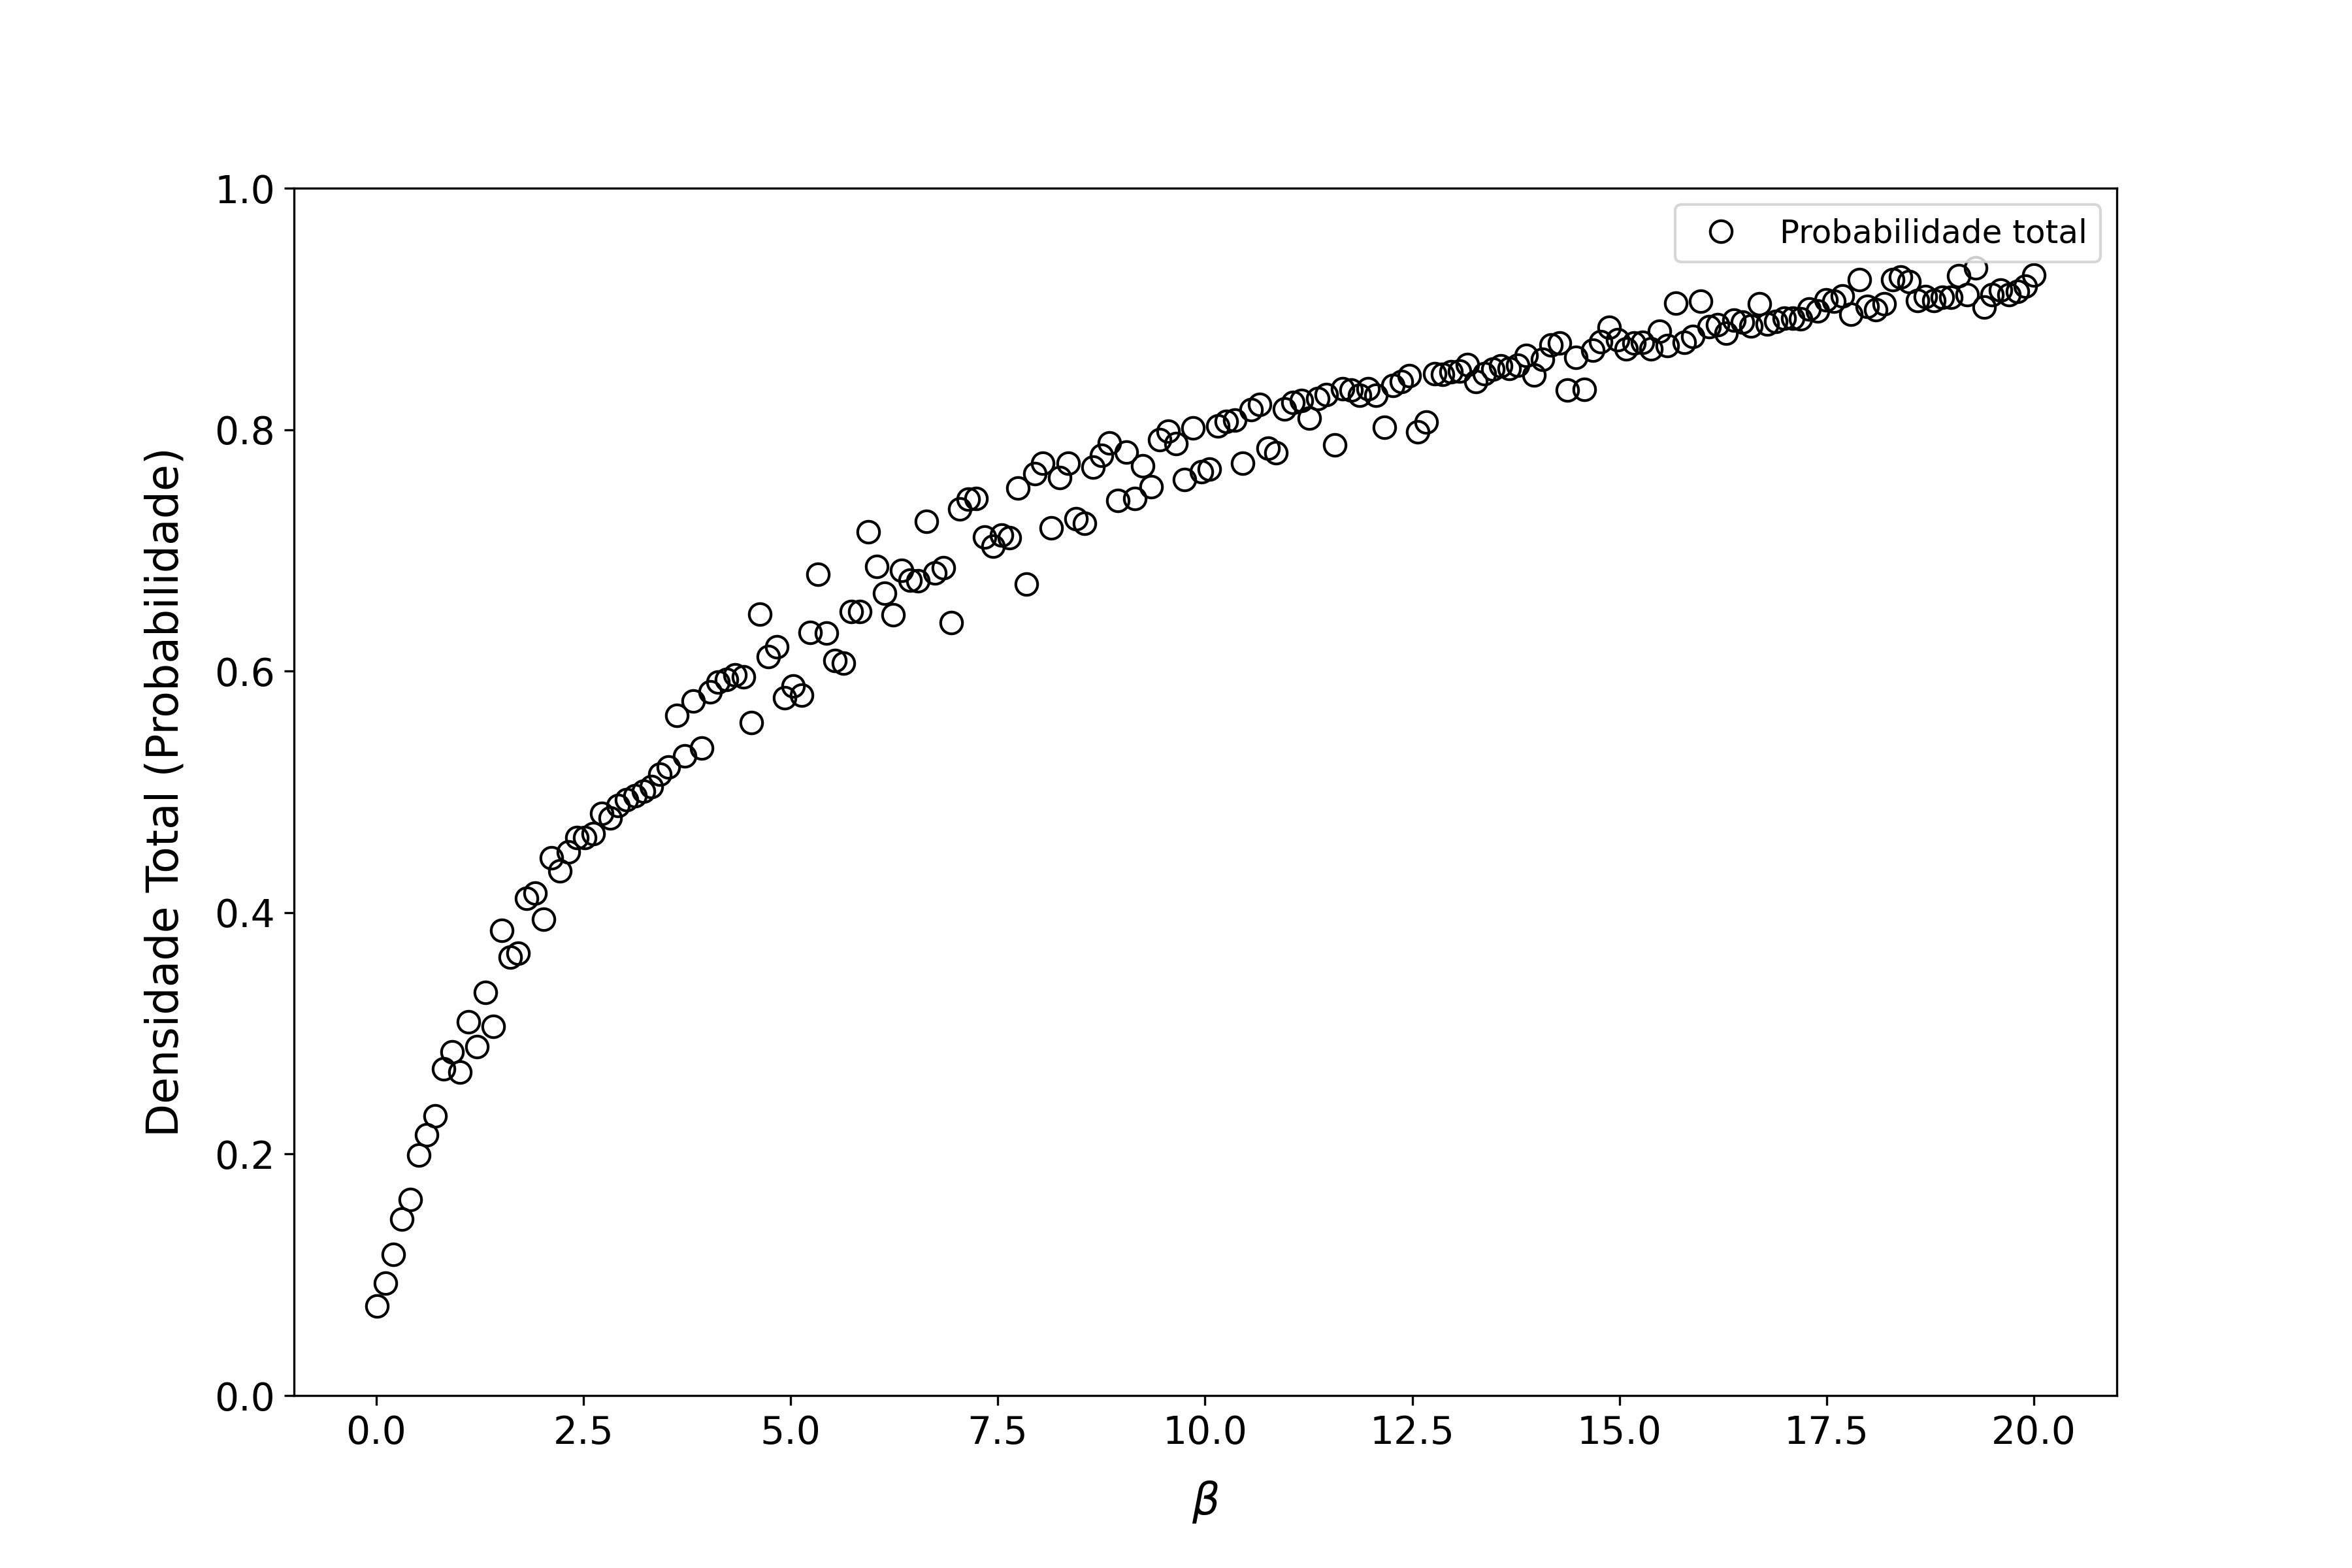
\includegraphics[scale=0.39]{Q2_d.png}
    \caption{Probabilidade de encontrar a partícula próxima aos mínimos em função do parâmetro \(\beta\).}
    \label{fig:Q2_d}
\end{figure}

\section*{Problema 2}
\section*{Problema 3}
Usando o importance sampling, conseguimos calcular o valor da integral. A amostragem se mostrou 
muito relevante para a exatidão do valor calculado. Para amostras entre \(1000\) e \(100000\), o erro
foi acima de \(1\%\). Para uma amostragem de \(1000000\) ou superior, o erro foi sempre inferior a \(1\%\),
mas o custo computacional tambem aumentou siginificativamente, indo de decimos para dezenas de segundos. 
Um dos melhores resultados que obtivemos foi:
\\

\noindent\textbf{Monte Carlo: 1.08049}\\
\textbf{Teórico: 1.08232}\\
\textbf{Erro: 0.1695}

\section*{Problema 4}
A solução para uma dimensão \(d\), dado que a integral não possui uma solução analítica, foi 
obtida utilizando uma calculadora de integrais e resulta em:

\begin{equation}
    \int_{[0,1]^d} f(x) \, dx = 0.7468^{d}.
\end{equation}

Com isso, para cada dimensão \(d\), calculamos numericamente o valor da integral e comparamos com o valor 
teórico. Os resultados obtidos, tomando a média para o máximo de amostragem em cada dimensão\((N = 200000)\), foram:

\begin{table}
    \centering
    \begin{tabular}{|c|c|c|}
        \hline
        Dimensão & Monte Carlo & Teórico \\
        \hline
        4 & 0.2764 & 0.2764 \\
        6 & 0.17346 & 0.17347 \\
        10 & 0.05396 & 0.05396 \\
        \hline
    \end{tabular}
    \caption{Comparação entre o valor da integral numérica e o valor teórico para cada dimensão.}
\end{table}

Ao analisarmos o erro absoluto entre o valor teórico e o valor obtido numericamente, observamos que 
ele apresenta uma relação direta com a dimensão do problema e com a necessidade de amostragem para 
atingir a convergência. Na Figura \ref{f1}, podemos observar os comportamentos. Para dimensões menores, é necessário um maior número de amostragens para 
que o erro converja para um valor muito pequeno. Em contrapartida, em dimensões maiores, uma menor 
quantidade de amostragens é suficiente para alcançar uma certa estabilidade do erro.
\begin{figure}[!htb]
    \centering
    % Linha superior: duas imagens lado a lado
    \begin{subfigure}{0.6\textwidth}
        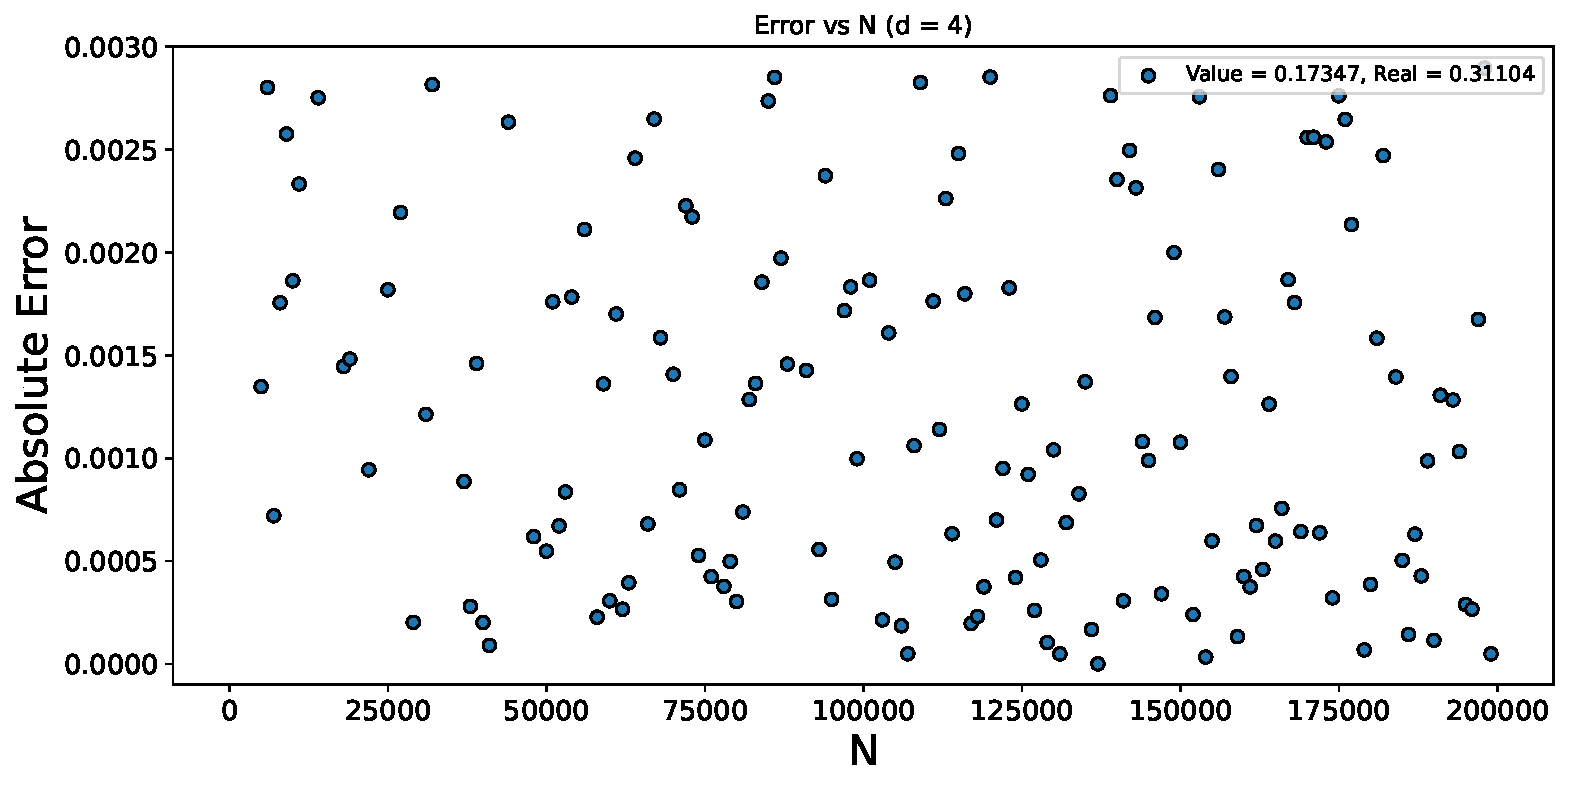
\includegraphics[width=\linewidth]{Q4.pdf}
        \caption{}
        \label{fig:subfig1}
    \end{subfigure}
    \hfill
    \begin{subfigure}{0.6\textwidth}
        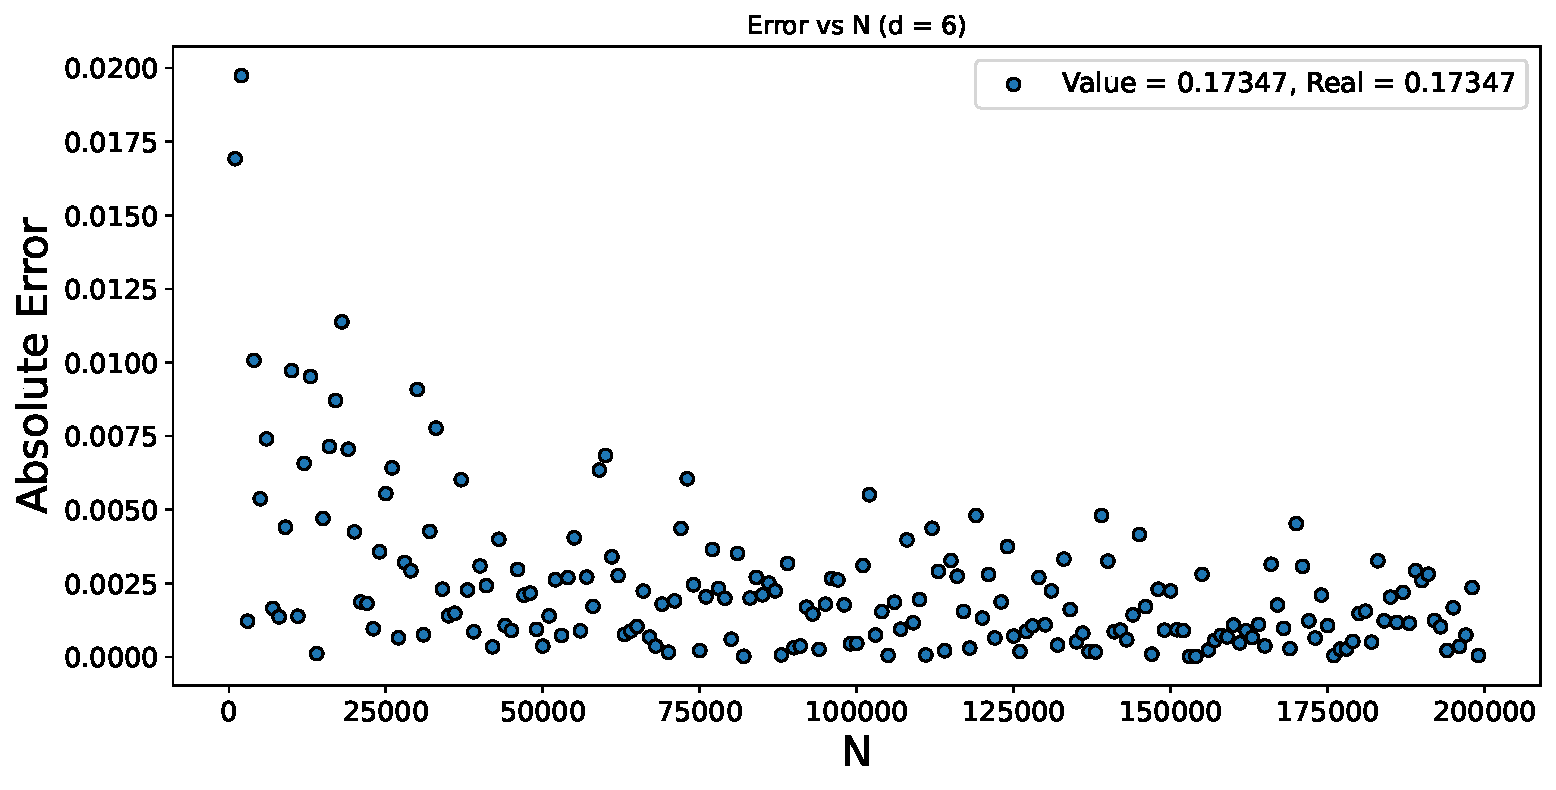
\includegraphics[width=\linewidth]{Q6.pdf}
        \caption{}
        \label{fig:subfig2}
    \end{subfigure}

    % Linha inferior: terceira imagem centralizada
    \vspace{0.5cm} % Espaçamento entre as linhas
    \begin{subfigure}{0.6\textwidth}
        \centering
        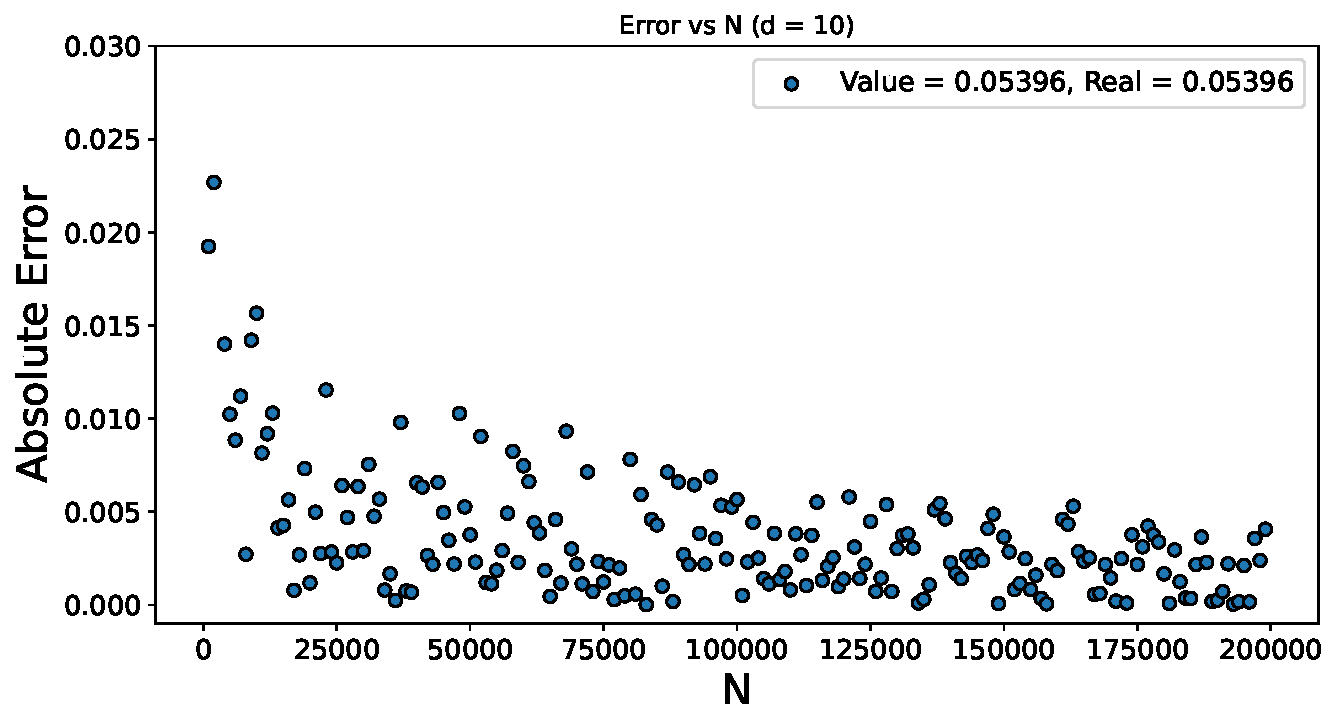
\includegraphics[width=\linewidth]{Q10.pdf}
        \caption{}
        \label{fig:subfig3}
    \end{subfigure}

    % Legenda geral
    \caption{Graficos do erro absoluto em função do número de amostragens para cada dimensão. 
    Na figura (a), temos d = 4, na figura (b), d = 6 e na figura (c), d = 10. Na legenda, temos
    o valor calculado da integral e o valor teórico.} 
    \label{f1}
\end{figure}

Por fim, analisando o erro em função da amostrage, fica mais facil observar, na Figura \ref{f2}
como a depencia da amostragem cai com o aumento da dimensão.

\begin{figure}[!htb]
    \centering
    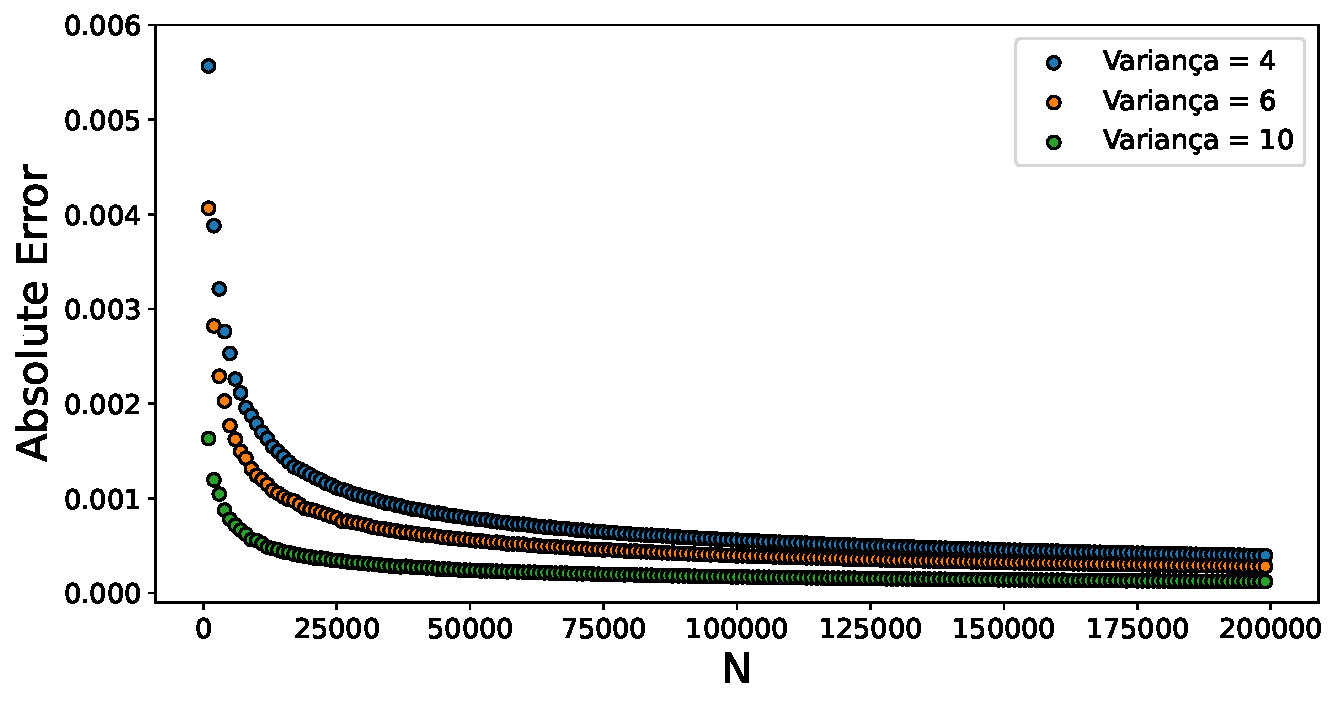
\includegraphics[width=0.6\textwidth]{erro.pdf}
    \caption{Erro em função do número de amostragens para as dimensões d = 4, 6, 10.}
    \label{f2}
\end{figure}

Por fim, para esse caso da integral, entender essa relação pode levar a uma diminuição do custo computacional
visto que para dimensões maiores, o número de amostragens necessárias é menor para uma boa solução.

\section*{Problema 5}

Iniciamos o problema gerando \(N = 200000\) amostras de uma distribuição uniforme entre \([0,\pi]\).
Nosso termo de aceite deveria ser algo da forma \(P(\theta) \propto 1 + \cos^2(\theta)\). Dessa 
forma, utilizamos a probabilidade de aceitação de uma amostra como sendo \(P(\theta) = 1 + M*
\cos^2(\theta)\), onde \(M = 0.05\). Com isso estabelecido, fizemos o histogram da distribuição de \(\theta\) e o 
normalizamos para poder comparar com a probabilidade teórica. Antes de realizarmos a comparação, 
realizamos uma integração numérica para obter o valor da constante de normalização. Sabendo que
a seguinte relação é valida, obtivemos como constante de normalização para \(P(\theta)\):

\begin{equation}
    C\int_{0}^{\pi} P(\theta) \, d\theta = 1,
\end{equation}
\begin{equation}
    C = \frac{1}{\int_{0}^{\pi} P(\theta) \, d\theta} = 0.2122.
\end{equation}

Na Figura \ref{f3}, temos a comparação entre a distribuição normalizada e a probabilidade 
\(P(\theta)\).
\begin{figure}[!htb]
    \centering
    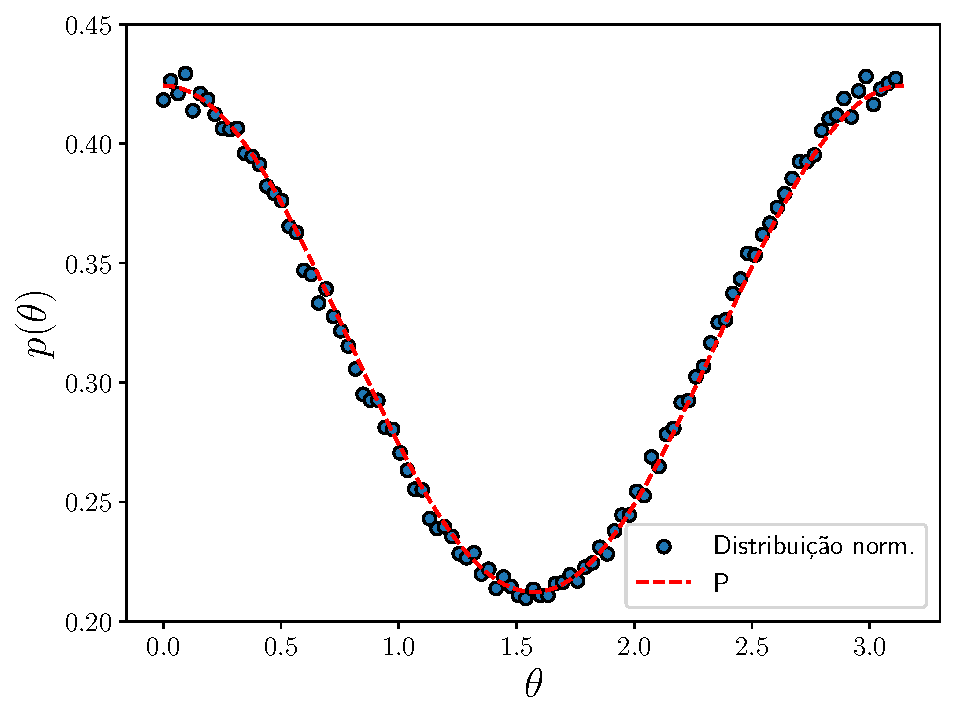
\includegraphics[width=0.6\textwidth]{distribuicao_theta_0.05.pdf}
    \caption{Comparação entre a distribuição normalizada e a probabilidade \(P(\theta)\).}
    \label{f3}
\end{figure}

Uma vez que conseguiamos com parar a distribuição normalizada com a probabilidade, nos buscamos 
a melhor forma de gerar a distribuição e estudamos como a constante \(M\) afetava a distribuição.
Nos observamos que para valores de \(M\) muito pequenos, a distribuição se tornava muito parecida 
com a probabilidade \(P(\theta)\). Na Figura \ref{f4}, temos a comparação entre a distribuição e 
a probabilidade para difentes valores de \(M\). Chegamos a conclusão que \(M < 1\) é a região que
começamos a igualar os dados.

\begin{figure}[!htb]
    \centering
    % Linha superior: duas imagens lado a lado
    \begin{subfigure}{0.48\textwidth}
        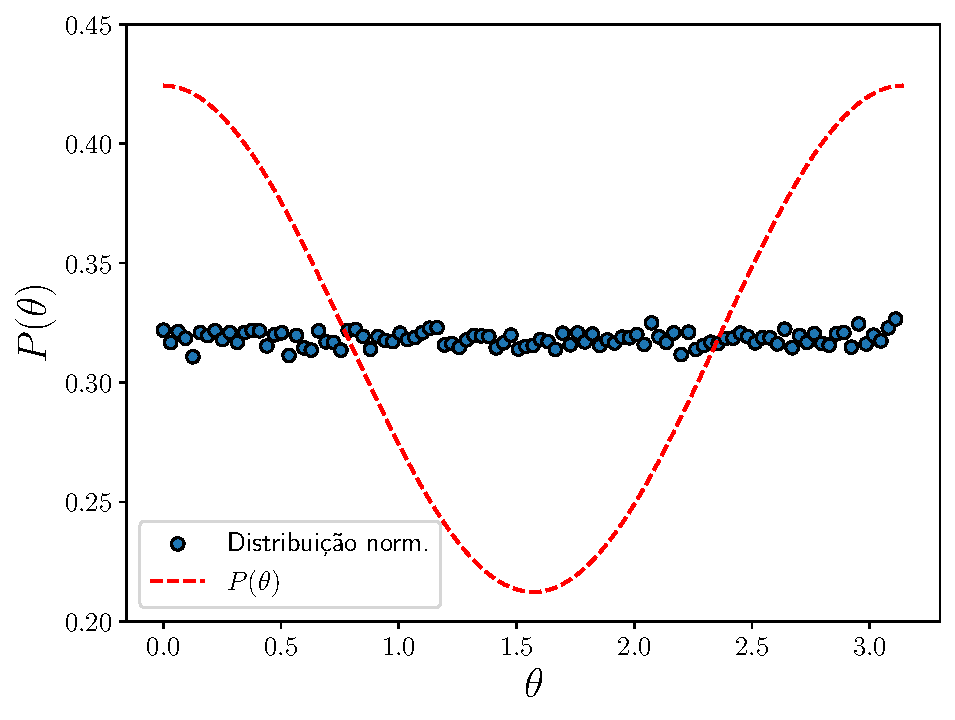
\includegraphics[width=\linewidth]{distribuicao_theta_5.pdf}
        \caption{}
        
    \end{subfigure}
    \hfill
    \begin{subfigure}{0.48\textwidth}
        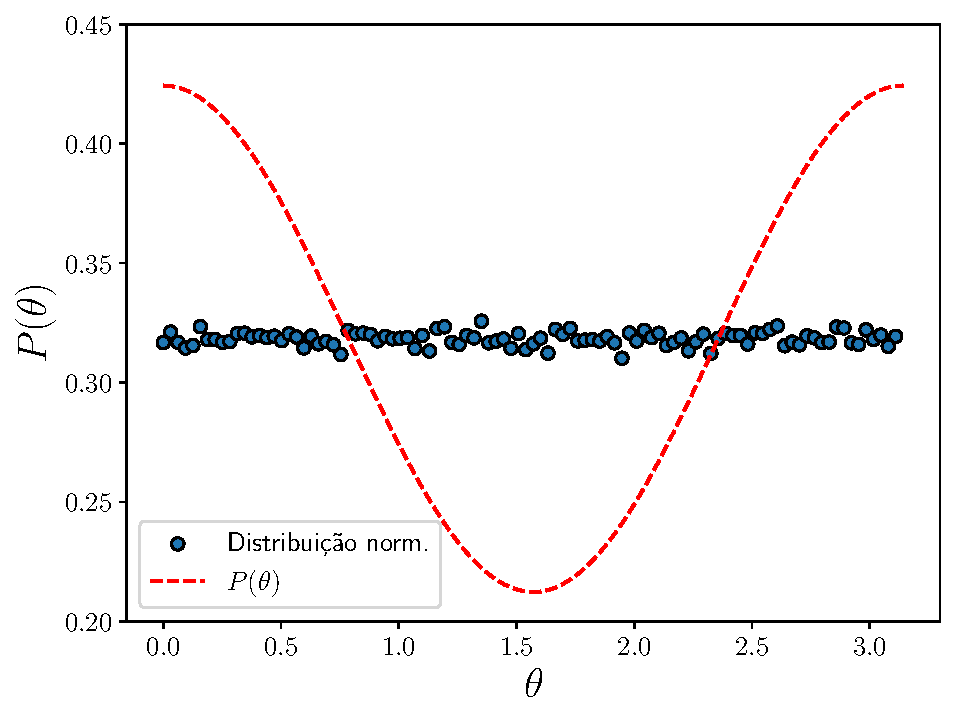
\includegraphics[width=\linewidth]{distribuicao_theta_1.pdf}
        \caption{}
        
    \end{subfigure}

    % Linha inferior: terceira imagem centralizada
    \vspace{0.2cm} % Espaçamento entre as linhas
    \begin{subfigure}{0.48\textwidth}
        \centering
        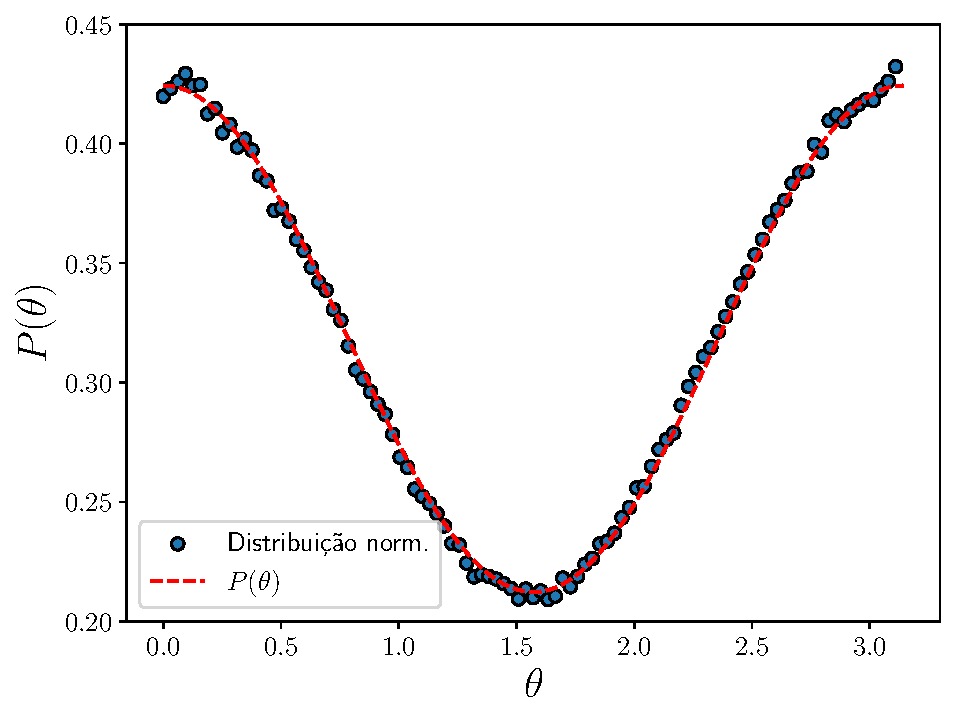
\includegraphics[width=\linewidth]{distribuicao_theta_0.1.pdf}
        \caption{}
      
    \end{subfigure}

    % Legenda geral
    \caption{Comparação entre a distribuição normalizada e a probabilidade \(P(\theta)\) para 
    diferentes valores de \(M\). Em (a), \(M = 5\), em (b), \(M = 1\) e em (c), \(M = 0.1\).} 
    \label{f4}

\end{figure}

Nosso próximo passo foi realizar testes estatisticos para comparar as distribuições. Primeiro 
calculamos a media e a variança as amostras em ambas as distribuições. Na Tabela \ref{t3} temos
os resultados obtidos. Ambas as métricas se mostraram praticamente, identicas nas duas distribuições.

\begin{table}
    \centering
    \begin{tabular}{|c|c|c|}
        \hline
        & Distribuição & \(P(\theta)\) \\
        \hline
        Média & 1.570796 & 1.572278 \\
        Variância & 0.989133 & 0.988647 \\
        \hline
    \end{tabular}
    \caption{Comparação entre a média e a variância das amostras para a distribuição e a probabilidade \(P(\theta)\).}
    \label{t3}
\end{table}

Por fim, realizamos um teste de Kolmogorov-Smirnov e qui-quadrado para comparar as distribuições. 
Os teste mostraram que as amostras de ambas as distribuições são praticamente identicas. Abaixo, temos
os resultados obtidos para os testes:
\\

\noindent\textbf{Kolmogorov-Smirnov Test:}\\
\textbf{Estatística D: }0.0043647\\
\textbf{Valor-p: }1.9961936
\\

Pela hipotese nula do teste de Kolmogorov-Smirnov, as distribuições são iguais, como o \(p> 0.05\),
ela não pode ser rejeitada, portanto, as distribuições são iguais.
\\

\noindent\textbf{Chi-Square Test:}\\
\textbf{Estatística Qui-Quadrado: }5448.6678171\\
\textbf{Valor-p: }1.0
\\

Pela hipotese nula do teste qui-quadrado, a amostra observada segue a distribuição teórica esperada, 
as distribuições são iguais, visto que \(p> 0.05\),
\end{document}
